\lab{Applications}{Point-to-Point Communication: The Trapezoidal Rule}{Parallelizing the Trapezoidal Rule}
\objective{Learn how to write basic parallel algorithms such as the trapezoidal rule}
\label{lab:MPI_Trapezoidal_Rule}

As was mentioned in the MPI Introduction lab \ref{lab:MPI_Intro}, the simplest message passing involves two processes: a sender and a receiver. In this lab, we will use these methods to parallelize the Trapezoidal Rule.

\section*{Simple Message Passing}
Let us begin by demonstrating a program designed for two processes. One will draw a random number and then send it to the other. We will do this using the routines \li{Comm.Send} and \li{Comm.Recv} (short for ``receive''):

\begin{lstlisting}
#passValue.py
import numpy as np
from mpi4py import MPI


COMM = MPI.COMM_WORLD
RANK = COMM.Get_rank()

if RANK == 1:  # This process chooses and sends a random value
    num_buffer = np.random.rand(1)
    print "Process 1: Sending: {num_buffer} to process 0.".format(**locals())
    COMM.Send(num_buffer, dest=0)
    print "Process 1: Message sent."
if RANK == 0:  # This process recieves a value from process 1
    num_buffer = np.zeros(1)
    print "Process 0: Waiting for the message... current num_buffer={num_buffer}.".format(**locals())
    COMM.Recv(num_buffer, source=1)
    print "Process 0: Message recieved! num_buffer={num_buffer}.".format(**locals())
\end{lstlisting}

To illustrate simple message passing, we have one process choose a random number and then pass it to the other. Inside the recieving process, we have it print out the value of the variable \li{num_buffer} \emph{before} it calls \li{Recv} to prove that it really is recieving the variable through the message passing interface.

Here is the syntax for \li{Send} and \li{Recv}, where \li{Comm} is a communicator object:

\begin{description}
\item[Comm.Send(buf, dest=0, tag=0)]
Performs a basic send. This send is a point-to-point communication. It sends information from exactly one process to exactly one other process.
Parameters:
\begin{description}
\item[buf (array-like)] – data to send.
    
    % TODO expand here- must be numpy array (as a pointer) and won't work with strings

\item[dest (integer)] – rank of destination
\item[tag (integer)] – message tag
\end{description}
Example:
\begin{lstlisting}
#Send_example.py
from mpi4py import MPI
import numpy as np

RANK = MPI.COMM_WORLD.Get_rank()

a = np.zeros(1, dtype=int)  # This must be an array
if RANK == 0:
    a[0] = 10110100
    MPI.COMM_WORLD.Send(a, dest=1)
elif RANK == 1:
    MPI.COMM_WORLD.Recv(a, source=0)
    print a[0]
\end{lstlisting} 
\item[Comm.Recv(buf, source=0, tag=0, Status status=None)]
Basic point-to-point receive of data.
Parameters:
\begin{description}
\item[buf (array-like)] – initial address of receive buffer (choose receipt location)
\item[source (integer)] – rank of source
\item[tag (integer)] – message tag
\item[status (Status)] – status of object
\end{description}
Example:
See example for Send()
\end{description}

\begin{info}
\li{Send} and \li{Recv} are referred to as \emph{blocking} functions. That is, if a process calls \li{Recv}, it will sit idle until it has received a message from a corresponding \li{Send} before it will proceeed. (However, the process that calls \li{Comm.Send} will \emph{not} necessarily block until the message is recieved- it depends on the implementation) There are corresponding \emph{non-blocking} functions \li{Isend} and \li{Irecv} (The \emph{I} stands for immediate). In essence, \li{Irecv} will return immediately. If a process calls \li{Irecv} and doesn't find a message ready to be picked up, it will indicate to the system that it is expecting a message, proceed beyond the \li{Irecv} to do other useful work, and then check back later to see if the message has arrived. This can be used to dramatically improve performance.
\end{info}

% TODO ASK is Send blocking in C? It isn't in python... I added in a note here

\begin{info}
When calling \li{Comm.Recv}, you can allow the calling process to accept a message from any process that happend to be sending to the receiving process. This is done by setting source to a predefined MPI constant, \li{source=ANY_SOURCE} (note that you would first need to import this with from \li{mpi4py.MPI import ANY_SOURCE} or use the syntax \li{source=MPI.ANY_SOURCE}).
\end{info}


\begin{problem}
Write a Python script \texttt{passVector.py} (adapted from \texttt{passValue.py}) that passes an $n$ by $1$ vector of random values from one process to the other. Write it so that the user passes the value of $n$ in as a command-line argument (similar to the code developed later in this lab for the trapezoidal rule).
\end{problem}

\begin{problem}
Try modifying some of the parameters in \li{Send} and \li{Recv} in the code from the previous exercise (\li{dest}, \li{source}, and \li{tag}).  What happens to the program? Does it hang or crash? What do you suppose the \li{tag} parameter does?
\end{problem}
% TODO delete this one?

\begin{problem}
Write a Python script \texttt{passCircular.py} (again adapted from \texttt{passValue.py}). This time, write the program so that each process with rank $i$ sends a random value to the process with rank $i+1$ in the global communicator. The process with the highest rank will send its random value to the root process. Notice that we are communicating in a ring. For communication, only use \li{Send} and \li{Recv}. The program should work for any number of processes. (Hint: Remember that \li{Send} and \li{Recv} are blocking functions. Does the order in which \li{Send} and \li{Recv} are called matter?)
% TODO \li{} for referencing file?
\end{problem}

\section*{The Trapezoidal Rule}
Now that we understand basic communication in MPI, we will proceed by parallelizing our first algorithm--numerical integration using the ``trapezoidal rule.'' Early on in most calculus classes, students learn to estimate integrals using the trapezoidal rule. A range to be integrated is divided into many vertical slivers, and each sliver is approximated with a trapezoid. The area of each trapezoid is computed, and then all their areas are added together.

% LaTeX to display the trapezoidal rule:
\begin{eqnarray*}%{rcl}
\textrm{Area} 
&\approx&
\sum_{i=0}^{n-1}\frac{[f(a+i \Delta x)+f(a + (i+1) \Delta x)]}{2}\cdot\Delta x \\
&=&
\left[-\frac{f(a)+f(b)}{2}+\sum_{i=0}^{n}f(a+i\Delta x)\right]\cdot\Delta x
\end{eqnarray*}
where $\Delta x=(b-a)/n$.

% Trapezoid rule picture:
\begin{figure}[h]
\centering
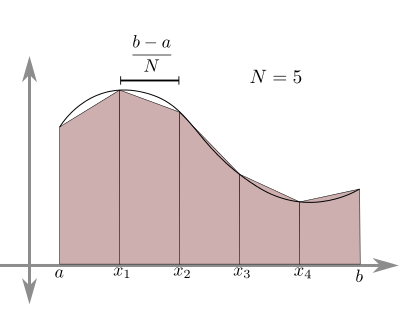
\includegraphics[width=.5\textwidth]{TrapezoidRule.png}
\caption{The trapezoid rule in action. TODO get a copyright-kosher version.}
\label{fig:trapezoidal_rule}
\end{figure}
% I took this template for icluding images from the data structures lab

In Python, a simple serial formulation of the trapezoidal rule would be as follows:

\lstinputlisting[style=fromfile]{trapSerial.py}

A moment of thought should convince the reader that this algorithm reflects the formula given above. 

\section*{Parallelizing the Trapezoidal Rule}
The first and most important step in parallelizing an algorithm is determining which computations are independent. With the trapezoidal rule, it's easy to see that the area of each trapezoid can be calculated independently, so dividing the data at the trapezoid level seems natural.

Currently, the algorithm divides up the interval into $n$ subintervals. To parallelize this process, we will distribute these $n$ subintervals to the available processes:

\lstinputlisting[style=fromfile]{trapParallel_1.py}

In this parallel approach, the original interval is split such that each process gets an equal-sized subinterval to integrate. After integrating, each process sends its result to the root node, which sums up the results and displays them. Although this is fairly straightforward, there are two important things to note:

First, notice how the trapezoids are divided among the processes: The processors each individually calculate the specifics of which subinterval they will be integrating. We could have written the algorithm such that process 0 divides up the work for the other processors and tells them each what their ranges are. However, this would introduce an unnecessary bottleneck: all of the other processes would be idling while waiting for their assignment to arrive from the root process. By having each process calculate its own range, we gain a large speedup.

Second, notice how the results are summed. We know how many results we should be receiving, so the root process simply accepts the messages in the order that they arrive. This is achieved using the tag \li{MPI.ANY_SOURCE} in the \li{COMM.Recv} method. In following labs we will learn about even more effective ways to gather the results of many different processes' computations.
% todo link to lab where we learn gather (next lab). Talk about the speed up we gained here? but in this case there is no speedup...

% MPI has two mechanisms specifically designed to partition the message space: tags and communicators. The tag parameter is there in the case that two messages with the same size and datatype are sent to the same process. In that case, the program would not necessarily be able to tell apart the data. So the programmer can attach different tags that he or she defines to the sent data to keep them straight.
% TODO find somewhere else for this paragraph to fit in maybe? Maybe as the answer to that problem from the intro that asks what tags do?

At this point, you should test the code for yourself. Save the code in a file named \texttt{trapParallel\_1.py} and try running it from the command line using the following input: 
\begin{lstlisting}[style=ShellInput]
$ mpirun -n 4 python trapParallel_1.py 0.0 1.0 10000
\end{lstlisting}
The output should appear like this:
\begin{lstlisting}[style=ShellOutput]
With 10000 trapezoids, our estimate of the integral of x^2 from 0.0 to 1.0 is:
    0.333333335
\end{lstlisting}
We have successfully parallelized our first algorithm!


\section*{Load Balancing}
Although we have parallelized the trapezoidal rule, our algorithm is still rather naive. Notice that if the number of processes does not evenly divide the number of trapezoids, the code will break down. Try running the trapezoid program with n = 10007 trapezoids:
\begin{lstlisting}[style=ShellInput]
$ mpirun -n 4 python trapParallel_1.py 0.0 1.0 10007
\end{lstlisting}
This will produce the following:
\begin{lstlisting}[style=ShellOutput]
With 10007 trapezoids, our estimate of the integral of x^2 from 0.0 to 1.0 is:
    0.333233404949
\end{lstlisting}

We know that the estimate of the integral should improve as $n$ grows larger, but this estimate is much worse. This happened because \li{local_n}, the number of trapezoids that each processor calculates, must be an integer. To solve this problem, we could require that the user always choose a value of $n$ that is divisible by the number of processors. However, good parallel code should let the user worry as little as possible about the parallelization and should function exactly as the serial version does. Thus, we should improve the code to let it handle the case where $n$ is not divisible by the number of processes.

One way to solve this problem would be to designate one process to handle the leftover trapezoids that; i.e. give each process \li{int(n/SIZE)} trapezoids and assign the remaining \li{n \% SIZE} trapezoids to the last process as well. Thus, the \li{local_n} of each process would be an integer. However, this method can be incredibly inefficient: What if we ran the program with $100$ processes and $n=1099$ trapezoids? Then each process would have \li{int(1099/100) = 10} trapezoids to calculate... except for the last process, which would have \li{10 + 1099 \% 100 = 109} trapezoids!

\emph{A parallel program can only be as fast as its slowest process.} We call this principle \emph{load balancing}. In this case, one process has to do over ten times as much work as the other processes! The other processes will end up waiting idle until the last one finishes. Ignoring communication costs and other overhead, this program could be nearly 10 times faster if we divided up the work more evenly. The important concept to remember is that any time a process is idling, we are losing efficiency.

In the case of the trapezoidal rule, load-balancing the code means two things. First, between any two processes, the number of trapezoids given to each must differ by at most $1$. Second, each process should estimate the area of a contiguous group of trapezoids. Although estimating an integral is not a very time-consuming operation, by estimating over contiguous groups of trapezoids we are minimizing the amount of duplicate work the processes have to do, which is good practice.

\begin{problem}
Implement the \emph{load-balancing} fix to the code \texttt{trapParallel\_1.py}. The program should be able to take in any number of trapezoids $n$ for any number of processes and the trapezoids should be divided among the processes evenly, differing by at most one between any two processes. Each process should independently calculate which section of trapezoids it should calculate.

For example, if the program is run with 5 processes and 12 trapezoids, processes 0 should calculate the first 3 trapezoids, process 1 should calculate the next 3 trapezoids, process 2 should calculate the next 2 trapezoids, process 3 should calculate the next 2 trapezoids, and process 4 should calculate the last 2 trapezoids.
\end{problem}
